Prabhāsa is a controlled, pre-registered evaluation of whether Pāṇinian morphosyntactic structure improves pretraining efficiency in small language models. It integrates morpheme and kāraka information via Vidyut morpheme-boundary embeddings and tests role-aware masking and an auxiliary objective against matched baselines on the BabyLM fixed-budget corpora (10M and 100M words) over BLiMP and GLUE.

\subsection{Architecture and Baseline}

The core model is a 14-layer Transformer encoder with hidden dimension 768, 12 attention heads, and feed-forward inner dimension 3072, comprising roughly 114M parameters on the Strict-Small (10M-token) budget and 100M parameters on the Strict (100M-token) budget after N-hot projection. Positional encoding uses Rotary Position Embedding (RoPE)~\cite{Su2021RoPE}, selected for compositional generalization, and the optimizer is Muon (Newton-Schulz orthogonalized momentum)~\cite{Jordan2024Muon}. The learning rate follows cosine annealing with 5\% warmup; each batch contains 256 sequences of maximum length 192 tokens. The pipeline is implemented in PyTorch with Hugging Face Transformers~\cite{Wolf2020Transformers}. Figure~\ref{fig:mechanism} summarizes the three Pāṇinian mechanisms.

\begin{figure}[t]\centering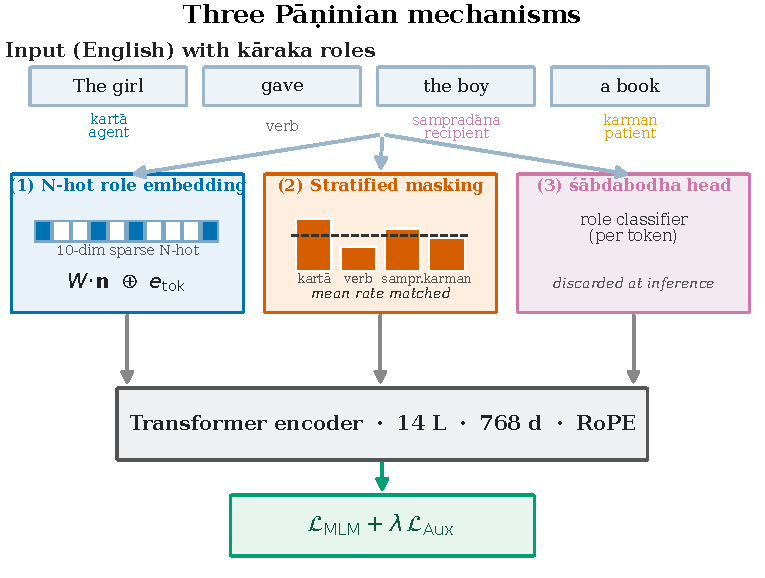
\includegraphics[width=\linewidth]{figures/fig_mechanism.pdf}
\caption{The three Pāṇinian mechanisms. (1) A Vidyut N-hot morpheme/role vector is projected and added to each token embedding; (2) kāraka role-stratified masking sets per-role mask probabilities whose mean is budget-matched to the uniform baseline; (3) a śābdabodha auxiliary head predicts kāraka roles from the encoder hidden state and is discarded at inference. The encoder is trained with $\mathcal{L}_{\text{MLM}} + \lambda\,\mathcal{L}_{\text{aux}}$.}
\label{fig:mechanism}\end{figure}

\subsection{Vidyut Embeddings, Kāraka Masking, and Auxiliary Objective}

For each token, Vidyut~\cite{Prasad2024Vidyut} produces a morpheme-boundary annotation and a kāraka-role label (kartā, karman, karaṇa, sampradāna, apādāna, adhikaraṇa, or a separator class). A sparse binary 10-dimensional vector encodes these and is projected to 768 dimensions and added to the token embedding, requiring no architectural change. The masking strategy adapts by role, $p_{\text{mask}}(t) = \alpha\,p_{\text{base}} + (1-\alpha)\,p_{\text{role}}(r(t))$, with per-role probabilities rescaled to hold the mean mask rate constant, so that any effect is attributable to the \emph{distribution} of masked tokens across roles rather than to total masked volume. The auxiliary objective predicts kāraka roles via a token-level head combined with the MLM loss at weight $\lambda$ (typically 1.0) and discarded before evaluation, so no role labels are needed at test time. See Appendix~\ref{app:training} for full configuration.

\subsection{Pretraining Objectives and Evaluation}

Two objectives are compared. The hybrid MLM\,+\,CLM configuration combines masked language modelling (15\% masked) with a causal next-token head weighted at 0.5; the pure-MLM configuration removes the CLM head. At the 10M-token budget the two are statistically indistinguishable (pure-MLM 63.58 $\pm$1.73 versus hybrid 64.09 $\pm$0.26 BLiMP, overlapping intervals); at the 100M-token budget pure-MLM reaches 73.06 against hybrid 67.57, a 5.49-point gap. The Strict-Small submission therefore retains the conservative hybrid objective, while the Strict track adopts pure-MLM. All models are evaluated on the official BabyLM suite: BLiMP~\cite{Warstadt2020BLiMP} (67 minimal-pair paradigms; primary metric multiple-choice accuracy), BLiMP Supplement, EWoK (Elements of World Knowledge)~\cite{Ivanova2024EWoK}, Entity Tracking, COMPS~\cite{Misra2023COMPS}, and GLUE~\cite{Wang2019GLUE}. Reported results are means with 95\% confidence intervals over three to five seeds (single seed for exploratory 100M arms); arm comparisons use paired bootstrap over per-paradigm subsets with Holm--Bonferroni correction. The Strict baseline is 74.53 BLiMP and the Strict-Small baseline 65.08~\cite{Hu2024BabyLM}.
